%%%%%%%%%%%%%%%%%%%%%%%%%%%%%%%%%%%%%%%%%%%%%%%%%%%%%%%%%%%%%%%%%%%%% 
%% This is a (brief) model paper using the achemso class 
%% The document class accepts keyval options, which should include 
%% the target journal and optionally the manuscript type. 
%%%%%%%%%%%%%%%%%%%%%%%%%%%%%%%%%%%%%%%%%%%%%%%%%%%%%%%%%%%%%%%%%%%%% 
\documentclass[journal=jctcce,manuscript=article]{achemso} 
 
%%%%%%%%%%%%%%%%%%%%%%%%%%%%%%%%%%%%%%%%%%%%%%%%%%%%%%%%%%%%%%%%%%%%% 
%% Place any additional packages needed here.  Only include packages 
%% which are essential, to avoid problems later. Do NOT use any 
%% packages which require e-TeX (for example etoolbox): the e-TeX 
%% extensions are not currently available on the ACS conversion 
%% servers. 
%%%%%%%%%%%%%%%%%%%%%%%%%%%%%%%%%%%%%%%%%%%%%%%%%%%%%%%%%%%%%%%%%%%%% 

%% Workaround for malfunctioning textsuperscript with pdfx and T1 encoding
\let\tmpa\textsuperscript
\DeclareTextCommandDefault{\textsuperscript}{\tmpa}

\usepackage[x11names]{xcolor}  % typesetting in color
%% Generate PDF/A-2u
%\usepackage[a-2u]{pdfx}
 
\usepackage[super]{natbib}         % citation style AUTHOR (YEAR), or AUTHOR [NUMBER]

\usepackage{achemso}  
\usepackage{rotating}  
%\usepackage{times} 
%\usepackage{lmodern}    %% Prefer Latin Modern fonts
\usepackage{graphicx} 
\usepackage{setspace} 
\usepackage{amsmath} 
\usepackage{epstopdf} 
\usepackage{csquotes} 
\usepackage{mhchem} 
\usepackage{chemfig} 
\usepackage[obeyFinal]{easy-todo}
\usepackage[english]{babel}
\usepackage{xr}
\externaldocument{manuscript}


\usepackage{subfig}
\usepackage{dcolumn}        % improved alignment of table columns
\usepackage{booktabs}       % improved horizontal lines in tables
\usepackage{paralist}       % improved enumerate and itemize

%% Character encoding: usually latin2, cp1250 or utf8:
\usepackage[utf8]{inputenc}
\usepackage[T1]{fontenc}

%\usepackage{markdown}  
 
%% The hyperref package for clickable links in PDF and also for storing
%% metadata to PDF (including the table of contents).
%% Most settings are pre-set by the pdfx package.
%\hypersetup{unicode}
%\hypersetup{breaklinks=true}
%\hypersetup{colorlinks,allcolors=DodgerBlue4}
 
%%%%%%%%%%%%%%%%%%%%%%%%%%%%%%%%%%%%%%%%%%%%%%%%%%%%%%%%%%%%%%%%%%%%% 
%% If issues arise when submitting your manuscript, you may want to 
%% un-comment the next line.  This provides information on the 
%% version of every file you have used. 
%%%%%%%%%%%%%%%%%%%%%%%%%%%%%%%%%%%%%%%%%%%%%%%%%%%%%%%%%%%%%%%%%%%%% 
%%\listfiles 
 
%%%%%%%%%%%%%%%%%%%%%%%%%%%%%%%%%%%%%%%%%%%%%%%%%%%%%%%%%%%%%%%%%%%%% 
%% Place any additional macros here.  Please use \newcommand* where 
%% possible, and avoid layout-changing macros (which are not used 
%% when typesetting). 
%%%%%%%%%%%%%%%%%%%%%%%%%%%%%%%%%%%%%%%%%%%%%%%%%%%%%%%%%%%%%%%%%%%%% 
\newcommand*\mycommand[1]{\texttt{\emph{#1}}} 
%%% Custom variables
% width suitable for fitting into a column in 1-column page layout
\newlength{\figwidth}
\setlength{\figwidth}{9 cm} 
\newlength{\figwidthsmall}
\setlength{\figwidthsmall}{6 cm} 
\newlength{\figwidthfull}
\setlength{\figwidthfull}{16 cm} 
\newlength{\figheightsmall}
\setlength{\figheightsmall}{6 cm} 
\newlength{\figheight}
\setlength{\figheight}{12 cm} 

 
%%%%%%%%%%%%%%%%%%%%%%%%%%%%%%%%%%%%%%%%%%%%%%%%%%%%%%%%%%%%%%%%%%%%% 
%% Meta-data block 
%% --------------- 
%% Each author should be given as a separate \author command. 
%% 
%% Corresponding authors should have an e-mail given after the author 
%% name as an \email command. Phone and fax numbers can be given 
%% using \phone and \fax, respectively; this information is optional. 
%% 
%% The affiliation of authors is given after the authors; each 
%% \affiliation command applies to all preceding authors not already 
%% assigned an affiliation. 
%% 
%% The affiliation takes an option argument for the short name.  This 
%% will typically be something like "University of Somewhere". 
%% 
%% The \altaffiliation macro should be used for new address, etc. 
%% On the other hand, \alsoaffiliation is used on a per author basis 
%% when authors are associated with multiple institutions. 
%%%%%%%%%%%%%%%%%%%%%%%%%%%%%%%%%%%%%%%%%%%%%%%%%%%%%%%%%%%%%%%%%%%%% 
 
\author{Josef Melcr} 
\email{melcr@marge.uochb.cas.cz} 
\affiliation[Czech Academy of Sciences]{Institute of Organic Chemistry and Biochemistry of the 
Czech Academy of Sciences, Flemingovo n\'{a}m. 542/2, CZ-16610 Prague 6, Czech Republic}
\alsoaffiliation{Groningen Biomolecular Sciences and Biotechnology Institute 
and The Zernike Institute for Advanced Materials, 
University of Groningen, 9747 AG Groningen, The Netherlands}

\author{Tiago Ferreira}
\affiliation{NMR group - Institut for Physics, Martin-Luther University Halle-Wittenberg} 
\author{Pavel Jungwirth} 
%%\homepage[]{http://jungwirth.uochb.cas.cz/}
\affiliation{Institute of Organic Chemistry and Biochemistry, 
Czech Academy of Sciences,  
Prague 6, Czech Republic} 
\author{O. H. Samuli Ollila} 
\email{samuli.ollila@helsinki.fi} 
%%\homepage[]{Your web page} 
\affiliation{Institute of Organic Chemistry and Biochemistry, 
Czech Academy of Sciences,  
Prague 6, Czech Republic} 
\alsoaffiliation{Institute of Biotechnology, University of Helsinki} 
 
 
%\author{Andrew N. Other} 
%\altaffiliation{A shared footnote} 
%\author{Fred T. Secondauthor} 
%\altaffiliation{Current address: Some other place, Othert\"own, 
%Germany} 
%\author{I. Ken Groupleader} 
%\altaffiliation{A shared footnote} 
%\email{i.k.groupleader@unknown.uu} 
%\phone{+123 (0)123 4445556} 
%\fax{+123 (0)123 4445557} 
%\affiliation[Unknown University] 
%{Department of Chemistry, Unknown University, Unknown Town} 
%\alsoaffiliation[Second University] 
%{Department of Chemistry, Second University, Nearby Town} 
%\author{Susanne K. Laborator} 
%\email{s.k.laborator@bigpharma.co} 
%\affiliation[BigPharma] 
%{Lead Discovery, BigPharma, Big Town, USA} 
%\author{Kay T. Finally} 
%\affiliation[Unknown University] 
%{Department of Chemistry, Unknown University, Unknown Town} 
%\alsoaffiliation[Second University] 
%{Department of Chemistry, Second University, Nearby Town} 
 
%%%%%%%%%%%%%%%%%%%%%%%%%%%%%%%%%%%%%%%%%%%%%%%%%%%%%%%%%%%%%%%%%%%%% 
%% The document title should be given as usual. Some journals require 
%% a running title from the author: this should be supplied as an 
%% optional argument to \title. 
%%%%%%%%%%%%%%%%%%%%%%%%%%%%%%%%%%%%%%%%%%%%%%%%%%%%%%%%%%%%%%%%%%%%% 
\title[] 
      { SUPPLEMENTARY INFORMATION: 
        Improved Cation Binding to Lipid Bilayer with
        Negatively Charged POPS by Effective
        Inclusion of Electronic Polarization
      }

%%%%%%%%%%%%%%%%%%%%%%%%%%%%%%%%%%%%%%%%%%%%%%%%%%%%%%%%%%%%%%%%%%%%% 
%% Some journals require a list of abbreviations or keywords to be 
%% supplied. These should be set up here, and will be printed after 
%% the title and author information, if needed. 
%%%%%%%%%%%%%%%%%%%%%%%%%%%%%%%%%%%%%%%%%%%%%%%%%%%%%%%%%%%%%%%%%%%%% 
%\abbreviations{IR,NMR,UV,MD,ECC,PC,PS,POPS,POPS} 
%\keywords{MD simulation, molecular modeling, 
%          polarizability, polarization,
%          phospholipids, phosphatidylserine} 

%%%%%%%%%%%%%%%%%%%%%%%%%%%%%%%%%%%%%%%%%%%%%%%%%%%%%%%%%%%%%%%%%%%%% 
%% The manuscript does not need to include \maketitle, which is 
%% executed automatically. 
%%%%%%%%%%%%%%%%%%%%%%%%%%%%%%%%%%%%%%%%%%%%%%%%%%%%%%%%%%%%%%%%%%%%% 

\renewcommand{\thetable}{S\arabic{table}}%
\renewcommand{\thefigure}{S\arabic{figure}}%
\renewcommand{\thesection}{S\arabic{section}}%
\renewcommand{\thepage}{S\arabic{page}}%


\begin{document} 

\clearpage
\section{Simulation details}
\begin{table}[!h]
  \caption{Simulation parameters}
  \label{tbl:mdpar}
  \begin{tabular}{ll}
    simulation property & parameter   \\
    \hline
    time-step           & 2~fs         \\
    equilibration time  & 50~ns  \\
    total simulation time     & $\geq 1 \mu$s  \\
    temperature         & 298~K       \\
    thermostat          & v-rescale  \cite{bussi07}   \\
    barostat            & Parrinello-Rahman, semi-isotropic \cite{parrinello81} \\
    long-range electrostatics & PME  \cite{darden93}  \\
    cut-off scheme      & Verlet \cite{Pall13}      \\
    Coulomb and VdW cut-off & 1.0~nm \\
    constraints         & LINCS, only hydrogen atoms \cite{hess97} \\
    constraints for water & SETTLE  \cite{miyamoto92} \\
    \hline
  \end{tabular}
\end{table}

\clearpage
\section{NMR experiments}

\begin{figure}[!h] 
  \centering 
  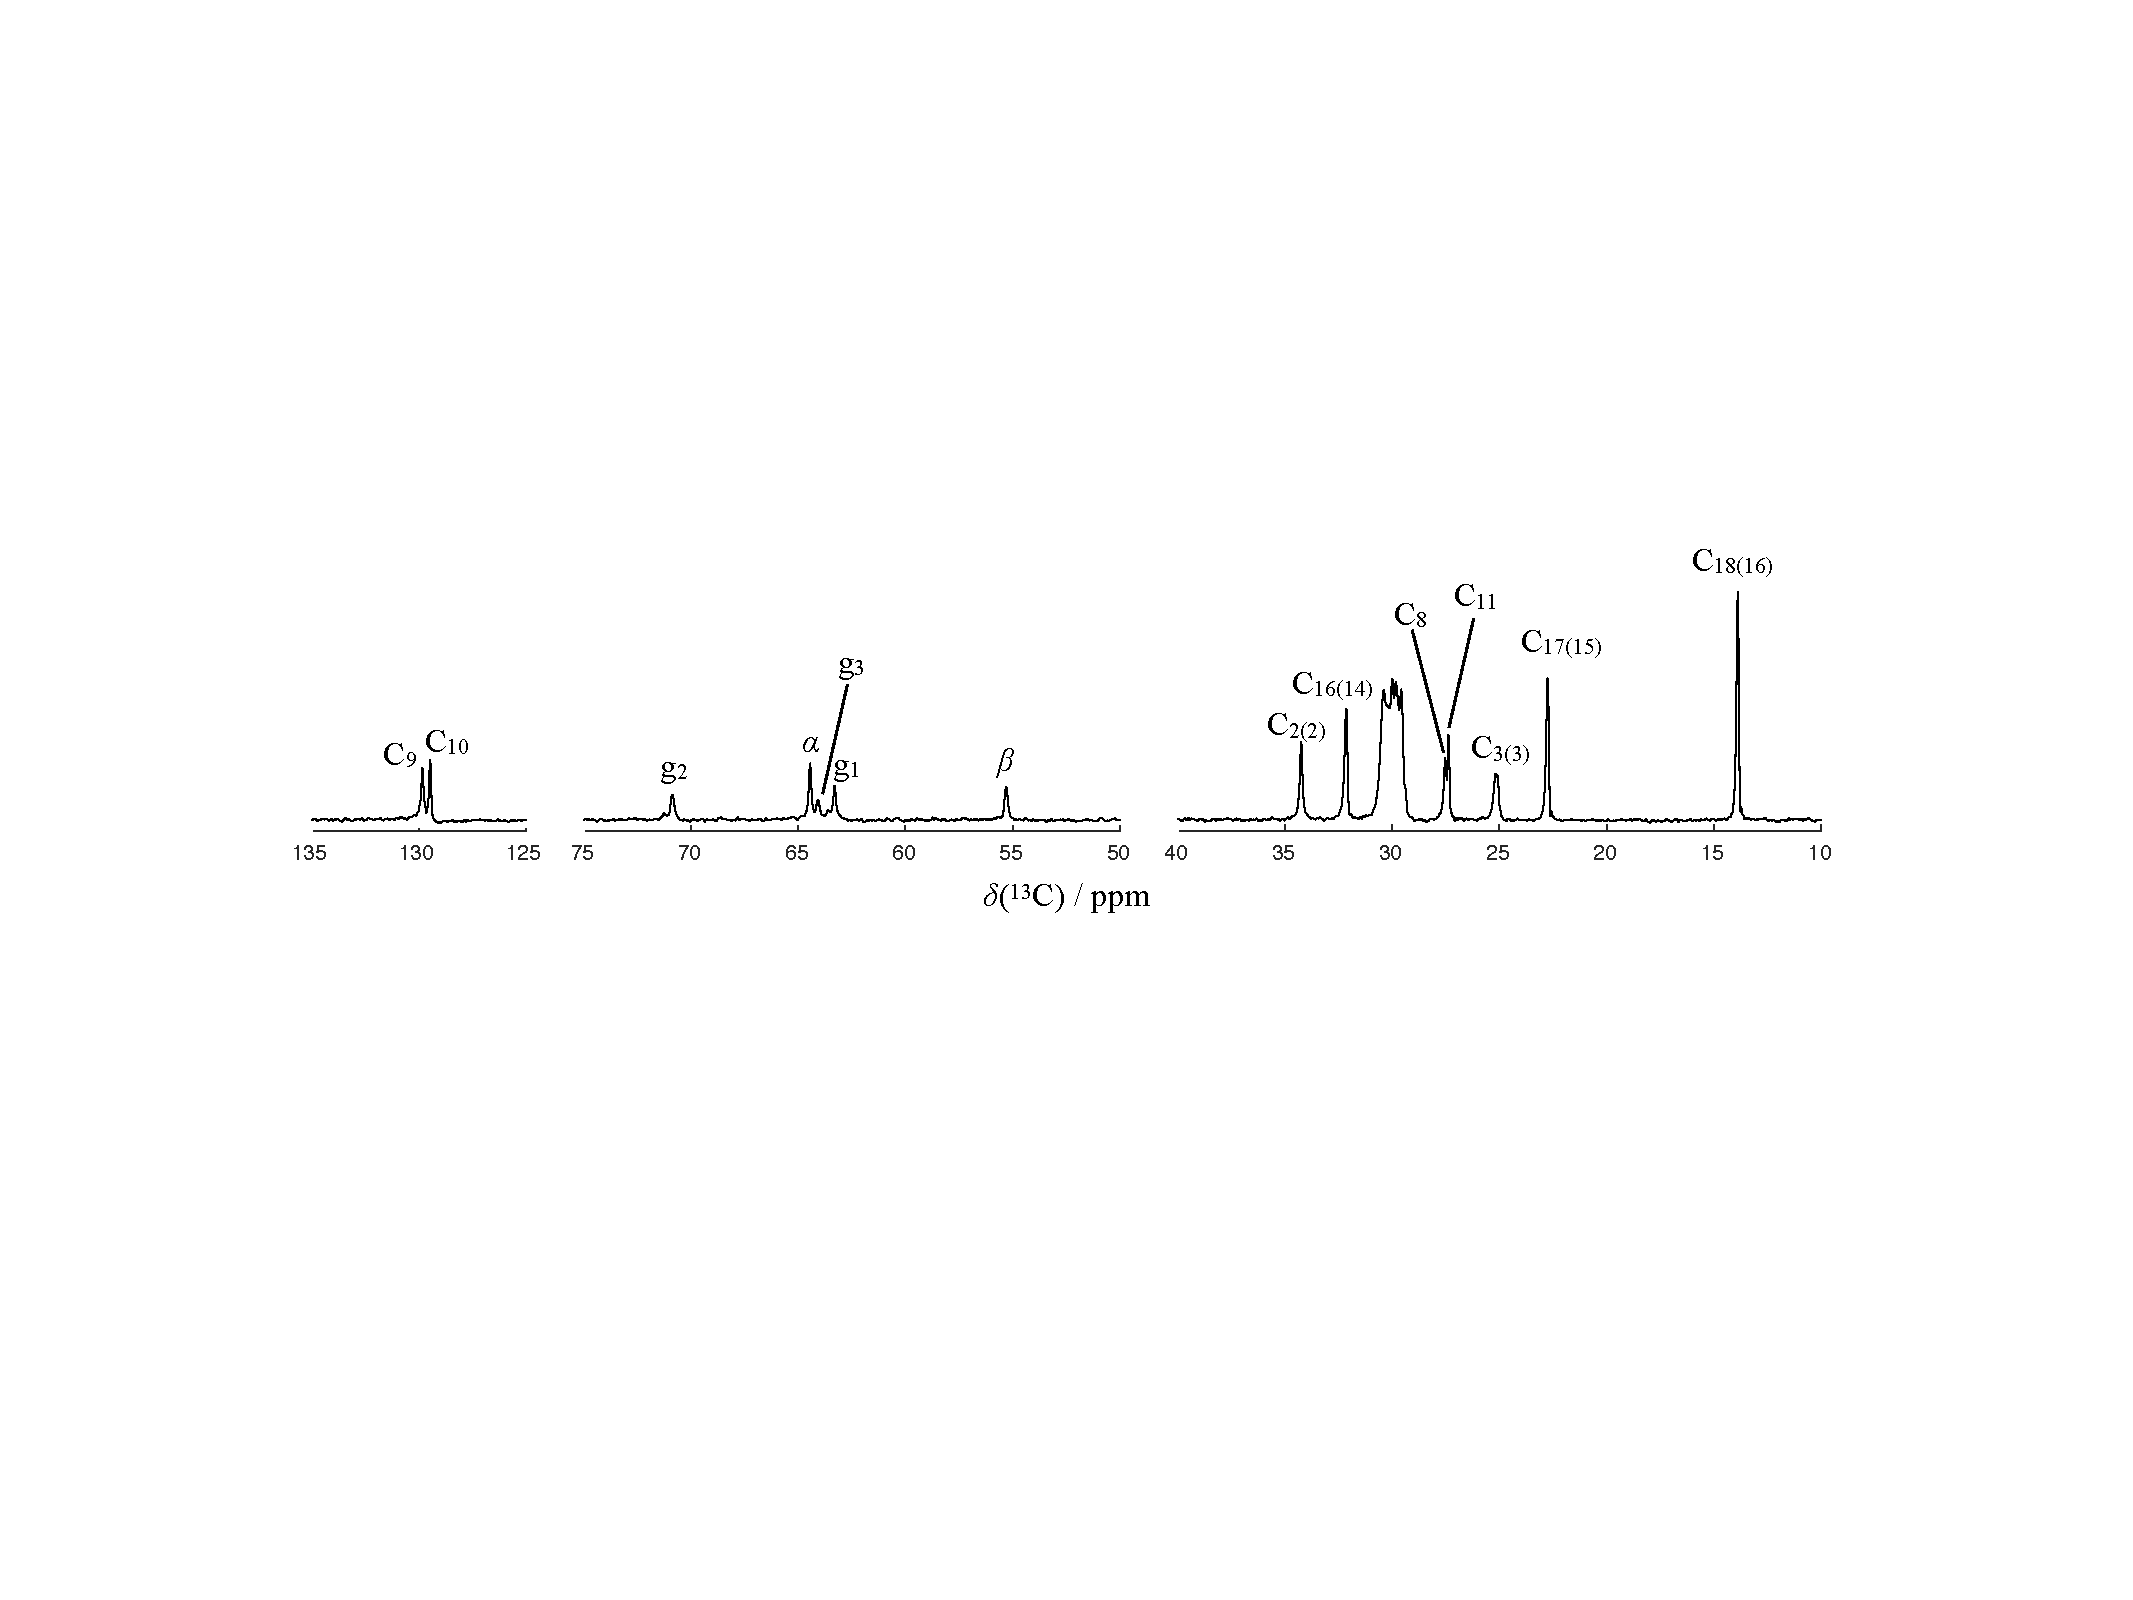
\includegraphics[width=\textwidth]{../Fig/POPSINEPT.pdf}
  \caption{\label{INEPT}
    Refocused-INEPT $^{13}$C spectrum of multilamellar POPS vesicles at 298 K
    with peak assignments for non--crowded spectral region ({\it sn}-1 chain in parenthesis).
  }
\end{figure}

\begin{figure}[!h] 
  \centering 
  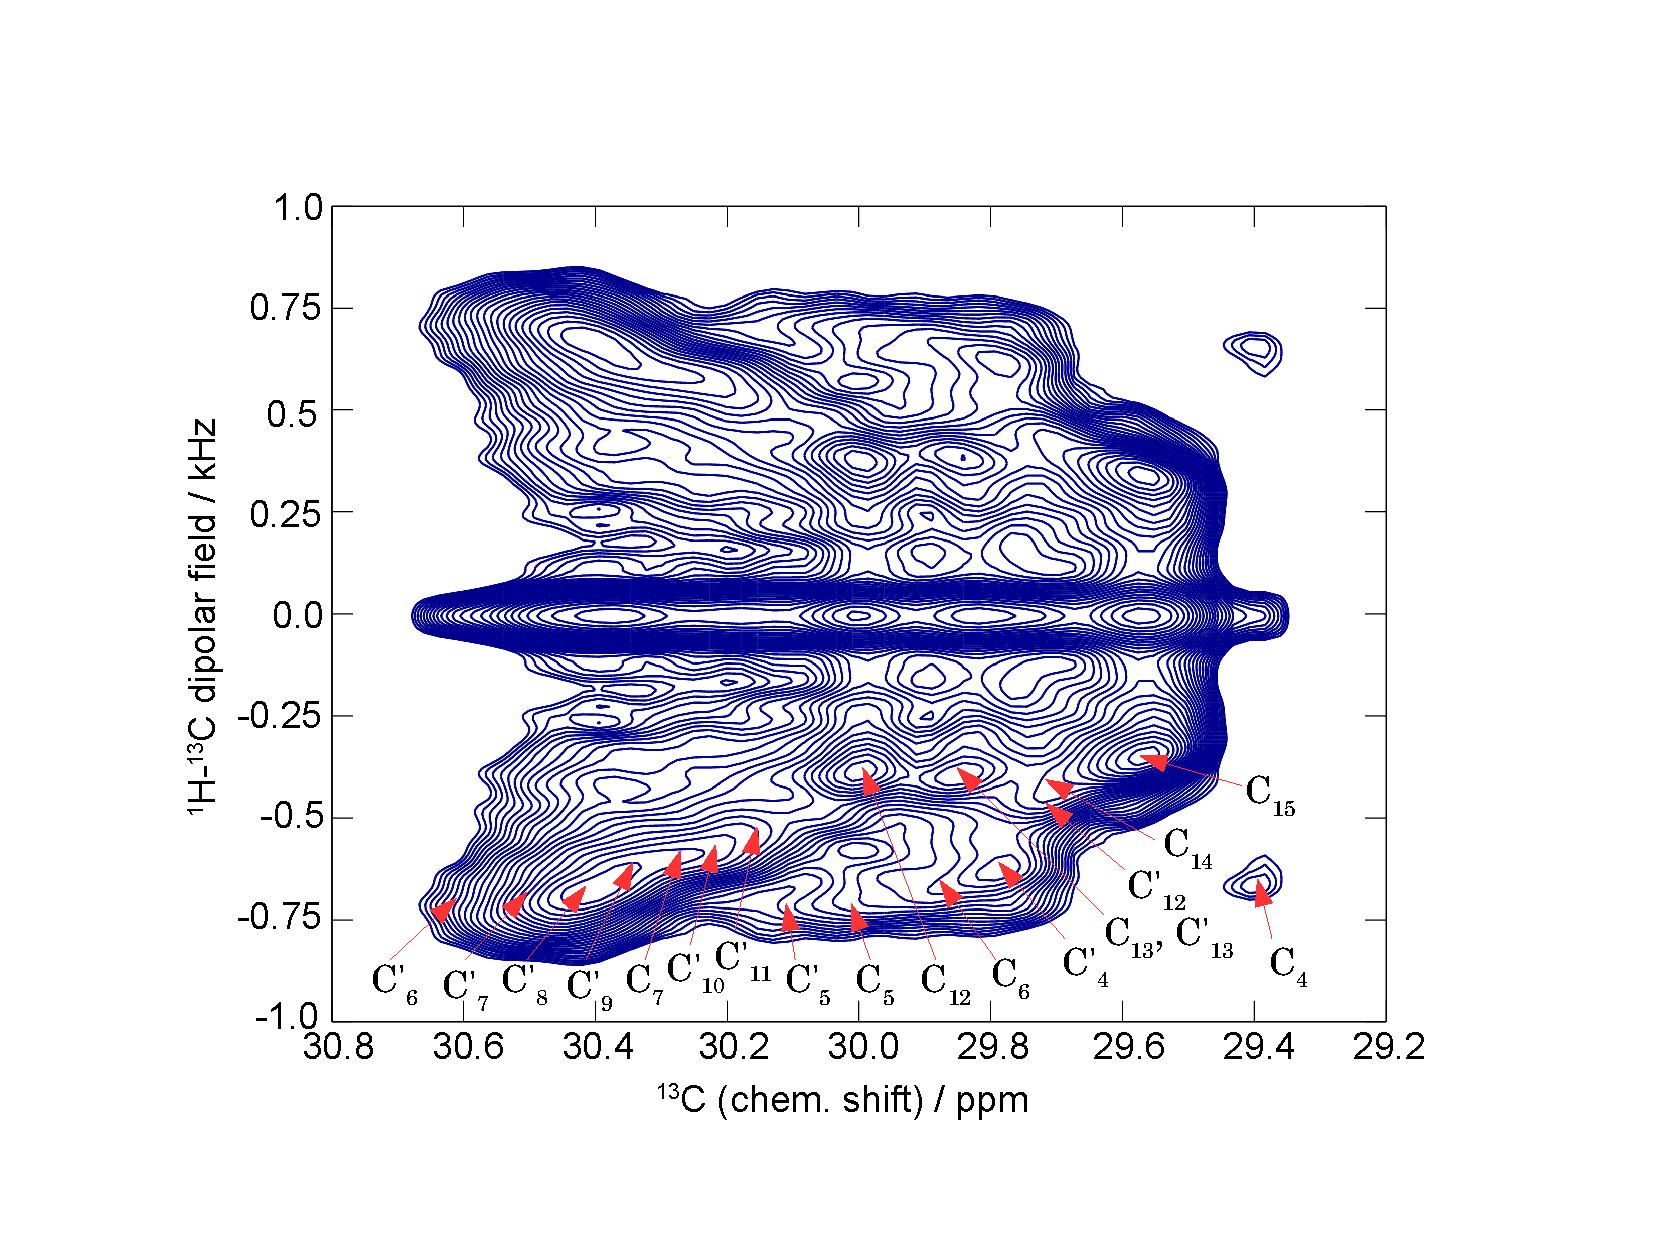
\includegraphics[width=\textwidth]{../Fig/crowded_region.pdf}
  \caption{\label{R-PDLF}
    2D-NMR R-PDLF spectra from the crowded spectral region of multilamellar POPS vesicles with the peak
    assignment. Apostrophes refer to the palmitoyl ({\it sn}-1) chain.
  }
\end{figure}

\begin{figure}[hbp!] 
  \centering 
  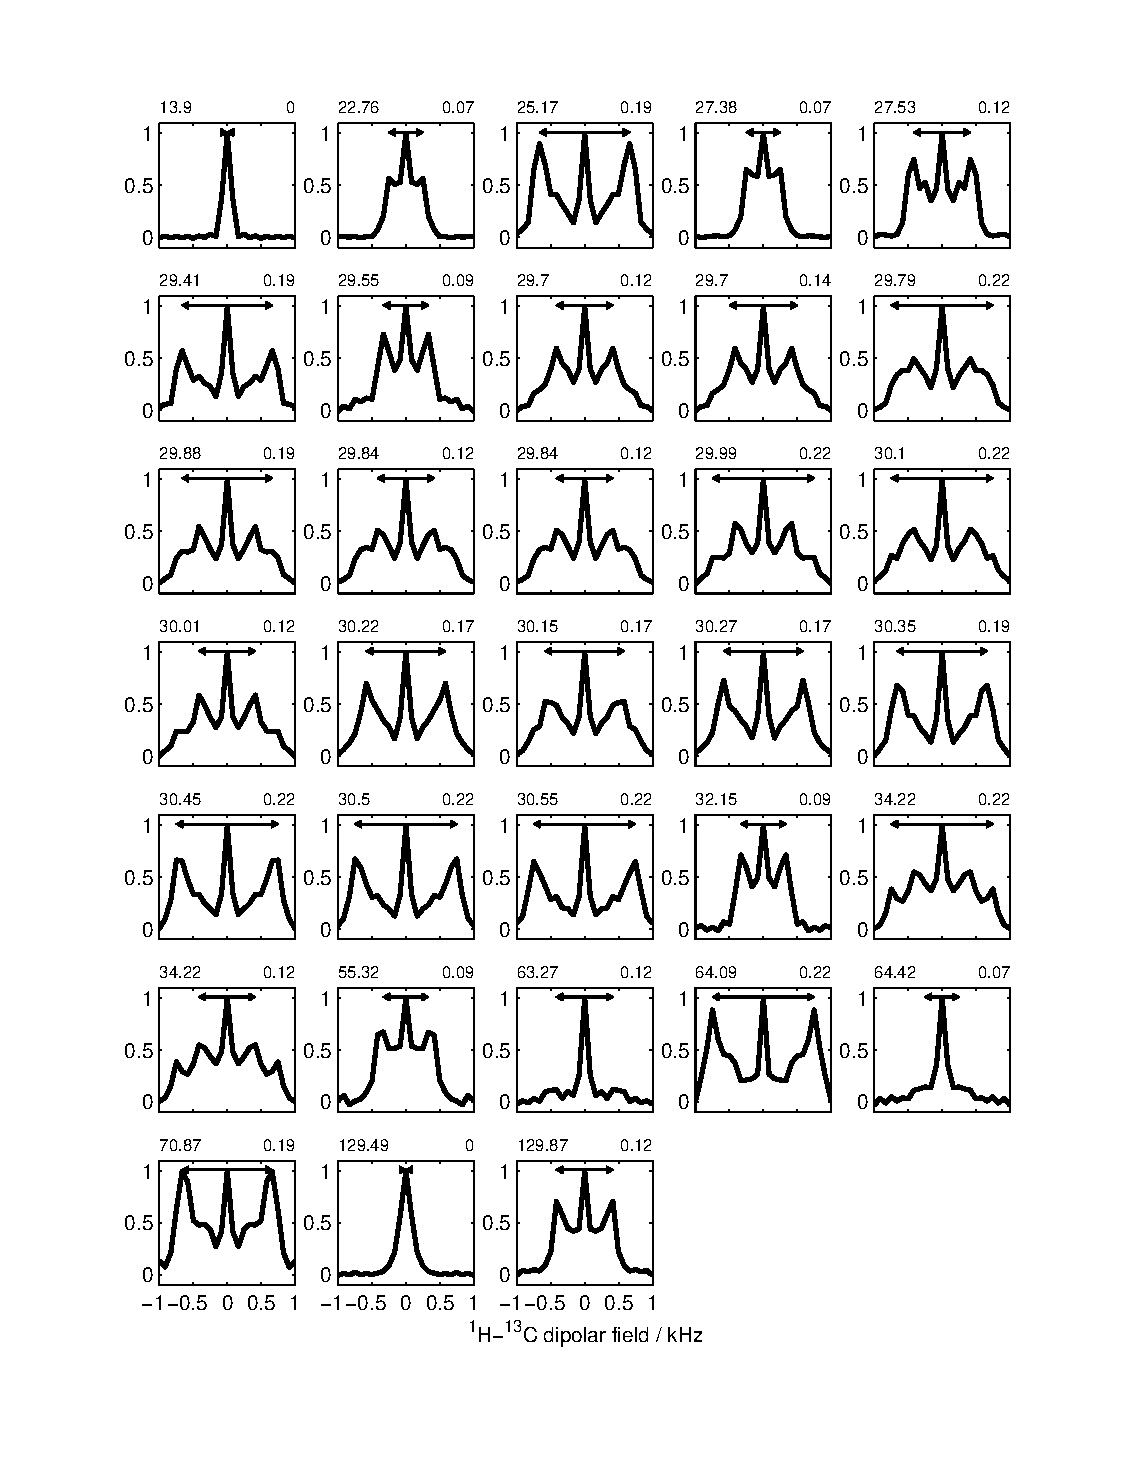
\includegraphics[width=\textwidth]{../Fig/slices_used.eps}
  \caption{\label{R-PDLFslices}
    Dipolar slices from the R-PDLF spectra of multilamellar POPS vesicles used to determine the acyl chain order parameters.
    Numbers of on top of figures refer to the chemical shift (left) and order parameter value (right).
  }
\end{figure} 


% SAMULI: I commented this out to simplify the manuscript
%
%\pagebreak
%
%\section{Distribution of dihedral angle \ce{C_\alpha-C_\beta-C_\gamma-O_\gamma} in POPS}
%\begin{figure}[hbp!] 
%  \centering 
%  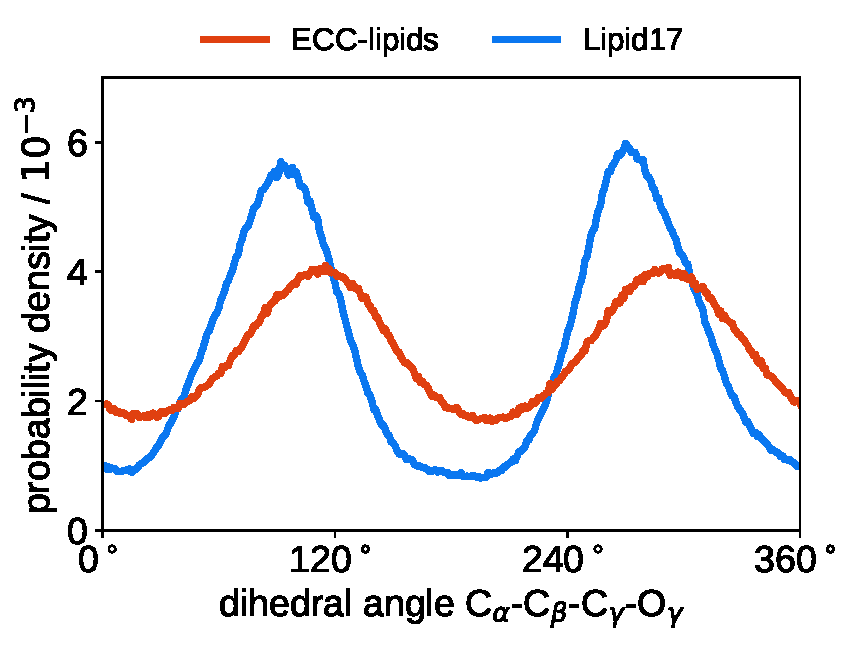
\includegraphics[width=\figwidth]{../img/dihedral_angle_distribution_Ca-Cb-Cg-Og_ECC-L17.pdf}
%  \caption{\label{fig:dihedral}
%    Distribution of dihedral angle \ce{C_\alpha-C_\beta-C_\gamma-O_\gamma} in POPS 
%    from simulations of a pure POPS bilayer with \ce{Na+} counterions using Lipid17 and ECC-lipids. 
%    Labelling of POPS segments is in Fig.~\ref{simVSexpNOions_POPS}. 
%}
%\todo{Cannot get rid of the copy of the Fig.1 cation}
%\end{figure} 


\pagebreak
\section{Interactions of POPS with \ce{K+} and \ce{Na+} counterions and POPC}

% SAMULI: I have moded the density profile figure in the main text
\begin{figure}[!h] 
  \centering 
  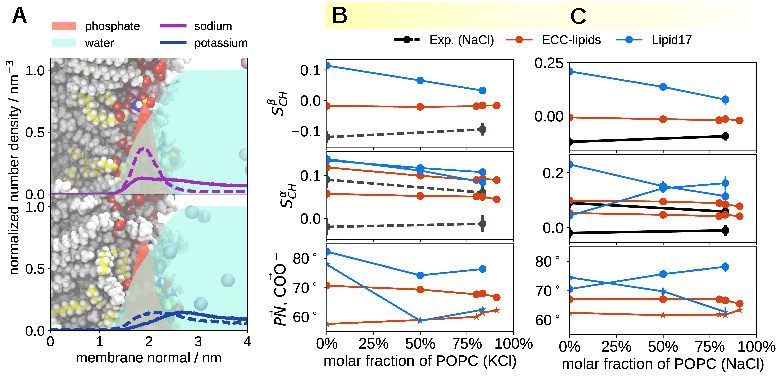
\includegraphics[width=\figwidthfull]{../img/deltaOP_mix_PC-PS_SupplInf-POPS-OP.pdf} 
  \caption{\label{fig:delta_ordPar_NaCl_PC-PS_mix_PS} 
    \textbf{(A)} Number density profiles of \ce{K^{+}} and \ce{Na^{+}} counterions along the membrane normal axis
    in ECC-lipids (solid lines) and Lipid17/Dang (dashed lines) simulations of POPC:POPS (5:1) bilayers.  
    The density profiles of phosphate groups and water are divided by 4 and 100, respectively.  
    \textbf{(B, C)} The POPS head group order parameters, the P--N (circles) and C$_\beta$--C$_\gamma$ vector angles (stars) 
    with respect to the membrane normal as a function of POPC content in a bilayer
    from ECC-lipids and Lipid17/Dang simulations with \ce{Na^+} (C) and \ce{K^+} (B) counterions.
    Experimental order parameter values are from Ref. \citenum{scherer87}
    and the signs from Ref.~\citenum{ferreira16} 
    (only \ce{Na^+} counterions, but shown also in the left plots (B) for \ce{K+} with dashed lines).
    Error bars are not visible for most of the simulation points because they are smaller than the point size.
    Chemical structure and labelling of carbon segments of POPC is shown in Fig.~\ref{fig:delta_ordPar_monoval_PCPS} in the main text. 
  }
\end{figure} 



\pagebreak

\section{Density profiles of additional monovalent cations in POPC:POPS (5:1) mixtures}

\begin{figure}[!h] 
  \centering 
  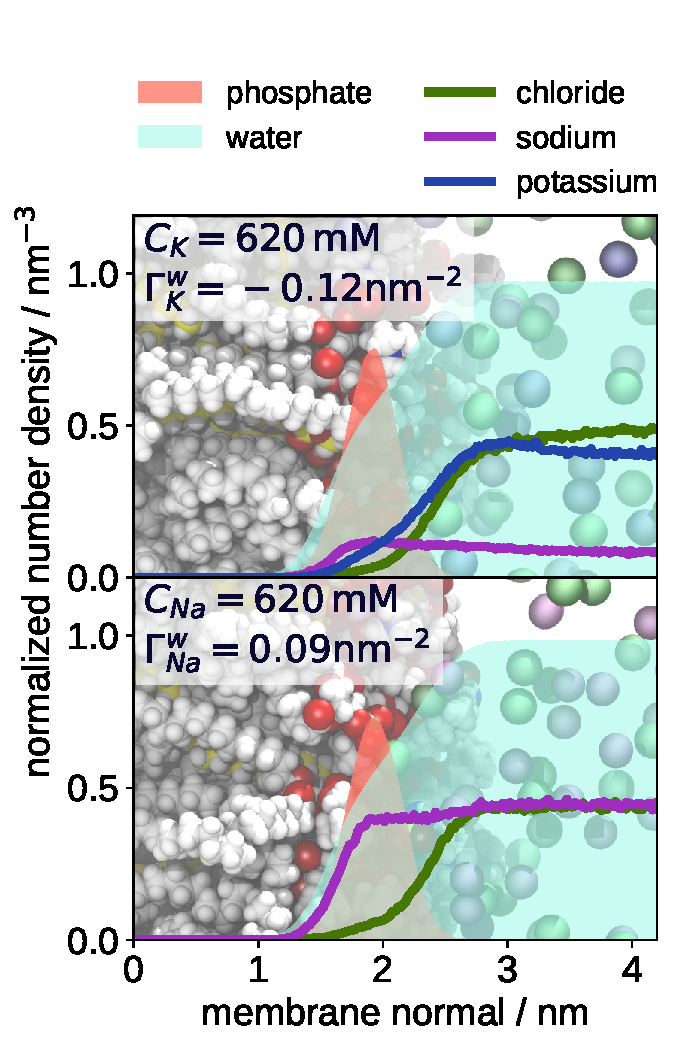
\includegraphics[width=\figwidth]{../img/ecc_pops/density_profiles_na_k_cl_wat_phos_models-compar_5-6_NaCl-and-KCl-series.pdf}
  \caption{\label{fig:nacl-dens_PCPS} 
    Number density profiles of \ce{K^{+}}, \ce{Na^{+}} and \ce{Cl^-} along the membrane normal axis
    from ECC-lipid simulation of POPC:POPS (5:1) mixture with \ce{Na^+} counterions and
    additional \ce{KCl} (top) and \ce{NaCl} (bottom) concentrations.
    The additional \ce{Na^+} are not distinguished from the counterions in bottom plot.
    The density profiles of phosphate groups and water are divided by 4 and 100, respectively.  
  }
\end{figure} 


\pagebreak




\section{Representative example configurations of \ce{Ca^{2+}} coordinated complexes with POPC and POPS phospholipids}

\begin{figure}[!h] 
  \centering 
  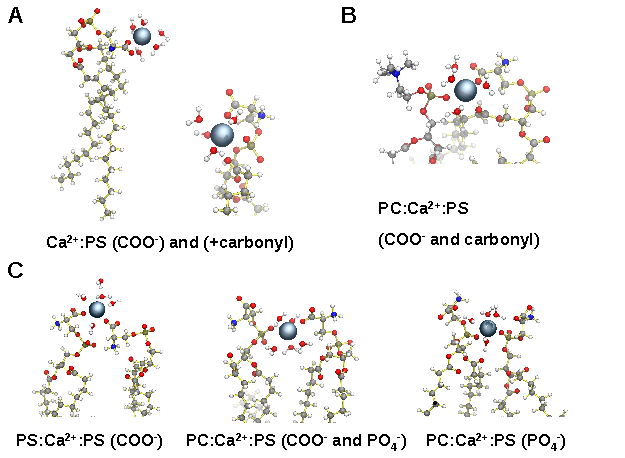
\includegraphics[width=\figwidthfull]{../img/populations_stoichiometry_structures_SI.pdf}
  \caption{\label{fig:strcutures_SI} 
    Representative example configurations of \ce{Ca^{2+}} coordinated complexes 
    of only one POPS (A), one POPS with one POPC (B) or two POPS lipids (C). 
    Probabilities of different calcium-phospholipid coplexes are shown in Fig.~\ref{fig:cacl_complexes} in the main text. 
  }
\end{figure} 


\pagebreak
\section{Populations of bound \ce{Ca^{2+}} cations to the PC:PS (5:1) bilayer}

\begin{table}[h!] 
\centering
\caption{%Bulk concentrations, $C _{Ca}$, and buffer concentrations, $C' _{Ca}$, of Ca$^{2+}$;
  % relative surface excess of calcium with respect to water ($\Gamma_{Ca}^{\rm water}$); 
  % and
  Percentages of the population of bound Ca$^{2+}$ to various lipid moieties in a pure POPC bilayer with 350 mM CaCl$_2$
  and in a POPC:POPS (5:1) mixture with 409 mM CaCl$_2$. The threshold for counting a contact was set to $0.3\,\mathrm{nm}$, which encompasses the
  first peak of the radial distribution function between the cations and the oxygen atoms of the lipids. 
  \label{tab:binding}} 
\begin{tabular}{ l | c c } 
 exclusive interacting moiety &  \multicolumn{2}{c}{percentage of bound \ce{Ca^{2+}} } \\
%	\hline
%	$C _{Ca}\,/\,\mathrm{mM}$  &  $240\pm 10 $  &  $280\pm 10 $  \\
%	$C'_{Ca}\,/\,\mathrm{mM}$  &  $400\pm 10 $  &  $350\pm 10 $  \\
%	$\Gamma_{Ca}^{\rm water}\, / \,\mathrm{nm}^{-2}$  &  $0.24 \pm 0.01 $  &  $0.06 \pm 0.01 $  \\
%	\hline
%                             &  \multicolumn{2}{c}{ } \\
                             &  5\,POPC:1\,POPS &  POPC   \\
    \hline
    \textbf{PC}              &   59   &  100   \\
	     PO$_4$    in PC &   41   &   67   \\
	     carbonyls in PC &   <1   &   ~1   \\
    \hline
    \textbf{PS}              &    8   &        \\ 
	     PO$_4$  in PS   &    2   &        \\
	     COO$^-$ in PS   &    4   &        \\
	     carbonyls in PS &   <1   &        \\
    \hline
    \textbf{both PC and PS}  &   33   &        \\
      PC and PO$_4$  in PS   &    9   &        \\
      PC and COO$^-$ in PS   &   17   &        \\
      PC and carbonyls in PS &   <1   &        \\
  \end{tabular} \\
\end{table} 


\pagebreak
\section{Residence times of cations}

% Already in the main text
%
%In ECC-lipid simulations, 90\% of the calcium residence times are shorter than $60\,\mathrm{ns}$ for pure POPC bilayer
%and shorter than $200\,\mathrm{ns}$ for POPC:POPS (5:1) mixture, while the
%longest observed residence times are $141\,\mathrm{ns}$ and $485\,\mathrm{ns}$, respectively (Fig.~\ref{fig:hist_residence_times}).
%The significantly shorter residence times in ECC-lipid simulations than in simulations 
%with other force fields~\cite{javanainen17, catte16} suggests that 1~$\mu$s simulations in this work
%are sufficiently long to equlibrate the ion concentration on lipid bilayer interface.
%Interestingly, the calcium residence times are 3-4 times longer in POPC:POPS (5:1) mixture than in
%pure POPC.

%Both estimates of the residence times come from simulations with comparable concentrations of around $250\mathrm{mM}$;
%the simulation with the neutral membrane has a bulk concentration of calcium $C_{ion} = 280\mathrm{mM}$, 
%whereas the simulation with the negatively charged membrane has a bulk concentration of calcium $C_{ion} = 240\mathrm{mM}$. 
%   In the simulation with the neutral membrane, 
%    90\% of the residence times of calcium cations are
%    shorter than $60\,\mathrm{ns}$, % exactly $53\,\mathrm{ns}$                                                                          
%    with the longest observed residence time being $141\,\mathrm{ns}$. 
%    In the simulation with the negatively charged membrane, 
%    90\% of the residence times of calcium cations are
%    shorter than $200\,\mathrm{ns}$, % exactly $53\,\mathrm{ns}$                                                                          
%    with the longest observed residence time being $485\,\mathrm{ns}$. 



\begin{figure}[!h]
  \centering
  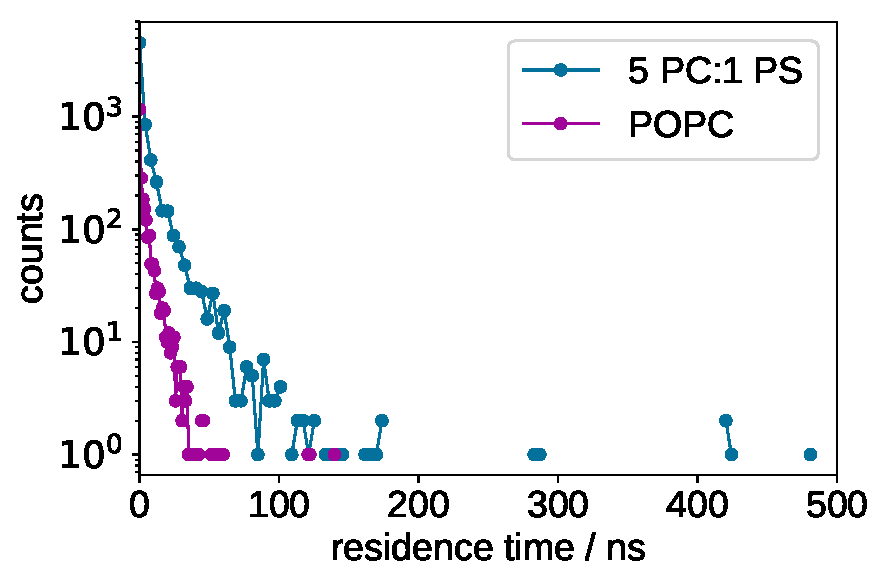
\includegraphics[width=\figwidth]{../img/histogram_bound_times_26CaCl2_comparison_PC-PCPS.pdf}
  \caption{\label{fig:hist_residence_times}
    Histograms of  \ce{Ca^{2+}} residence times in a pure POPC with 350 mM CaCl$_2$
    and in a POPC:POPS (5:1) mixture with 400 mM CaCl$_2$ from ECC-lipid simulations.
    %The simulation with the neutral membrane has a bulk concentration of calcium $C_{ion} = 280\mathrm{mM}$, 
    %the simulation with the negatively charged membrane has a bulk concentration of calcium $C_{ion} = 240\mathrm{mM}$. 
    Previously published simulation data \cite{melcr18} for pure POPC bilayers was taken directly from Ref.~\citenum{ECC-POPC_nacl_cacl2_files}.
  }
\end{figure}



\bibliography{refs.bib} 
 
\end{document} 
 

